\chapter{Registerallocatie}
Graph coloring om registers te alloceren in een interference graph.


Met sommige knopen geen rekening houden (bv h, want er zullen toch twee kleuren overblijven want heeft maar 2 buren).

\begin{enumerate}
	\item Vereenvoudig de graaf door continue knopen met een graad $< k$ weg te laten. Steek ze op een stack.
	\item Pop and color: selecteer een kleur en voeg knoop terug toe met die kleur aan de graaf.
\end{enumerate} 

\section{Register Coalescing}
Knopen die kopieën bevatten proberen samen te voegen als die het kleuren hoogstwaarschijnlijk niet bemoeilijken.

Twee heuristieken die het kleuren zeker niet moeilijker maken:
\begin{itemize}
	\item heuristiek van Briggs: als samengevoegde knoop minder dan $K$ buren van significante graad heeft
	\item heuristiek van George: Elke buur $t$ van $a$ is ofwel een buur van $b$ ofwel niet van significante graad.
\end{itemize}

Figuur \ref{fig:graph_coalescing} illustreert het algoritme en bestaat uit een aantal operaties.

\begin{figure}
	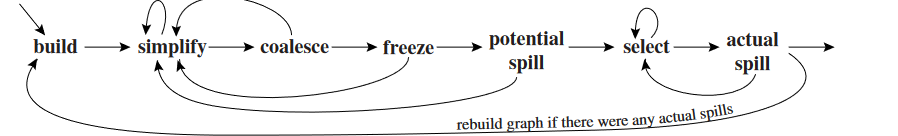
\includegraphics[width=\textwidth]{graph_coalescing}
	\caption{Graafkleuring met \textit{coalescing}.}
	\label{fig:graph_coalescing}
\end{figure}

\begin{itemize}
	\item \textbf{Build:} Construeer de interferentiegraaf en markeer elke knoop als \textit{move-related} of \textit{non-move-related}. Een \textit{move-related} knoop is een knoop dat ofwel het doel of de bron is van een \textit{move} instructie.
	\item \textbf{Simplify:} Verwijder iteratief één \textit{non-move-related} knoop die  graad minder dan $K$ heeft.
	\item \textbf{Coalesce:} Pas \textit{conservative coalescing} toe op de gereduceerde graaf met behulp van Briggs of George. \textbf{Simplify} en \textbf{Coalesce} wordt uitgevoerd tot dat er 
	\item \textbf{Freeze:}
	\item \textbf{Potential Spill:}
	\item \textbf{Select:}
	\item \textbf{Actual spill:}
\end{itemize}